\chapter{Behavior \ooad[91]}\label{chapter:behavior}
\begin{figure}[H]
    \begin{tabular}{|l|p{12cm}|}
        \hline
        \textbf{Purpose} & \begin{itemize}
            \item To model the dynamics of a problem domain
        \end{itemize} \\\hline
        \textbf{Concepts} & \begin{itemize}
            \item Event trace: A sequence of events involving a specific object.
            \item Behavioral pattern: A description of possible event traces for all objects in a class.
            \item Attribute: A descriptive property of a class or an event.
        \end{itemize} \\\hline
        \textbf{Principles} & \begin{itemize}
            \item Create behavioral patterns from event traces.
            \item Study common events.
            \item Derive class attributes from behavioral patterns.
        \end{itemize} \\\hline
        \textbf{Result} & \begin{itemize}
            \item A behavioral pattern with attributes for every class in a class diagram.
        \end{itemize} \\\hline
    \end{tabular}
\end{figure}

\begin{figure}[H]
    \centering
    \includegraphics*[width=\linewidth]{parts/2_problem_domain_analysis/behavior/figures/structure_activity.png}
\end{figure}

\section{Behavioral Pattern and Attributes}
In the behavior activity the behavior is described more precisely by adding relative timings to events. Object behavior is defined by an event trace, that exhibits a certain ordering of events.

\subsection*{Event trace \ooad[92]}
\begin{figure}[H]
    \textit{\textbf{Event trace -} A sequence of events involving a specific object}
\end{figure}

An event trace is unique for a single object. It's the precise sequence in a time interval.\\
\\
Birth $\rightarrow$ event\_1 $\rightarrow$ event\_2 $\rightarrow$ $\cdots$ $\rightarrow$ event\_n $\rightarrow$ death.

\subsection*{Behavioral pattern \ooad[92]}
\begin{figure}[H]
    \textit{\textbf{Behavioral pattern -} A description of possible event traces for all objects in a class.}
\end{figure}
To produce the pattern, examples of event traces for individual objects in a class are used. For problem-domain dynamics, the object collaboration is emphasized; study common events. Common events are used to describe interactions between classes.

\section{Notation for Behavioral Patterns}
\begin{itemize}
    \item (+) Sequence: Events in a set occur one by one.
    \item ($\vert$) Selection: Exactly one out of a set of events occurs.
    \item (*) Iteration: An event occurs zero or more times.
\end{itemize}

\begin{figure}[H]
    \centering
    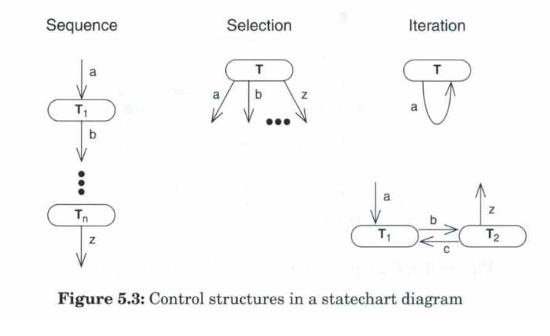
\includegraphics[width=\linewidth]{parts/2_problem_domain_analysis/behavior/figures/statechart.png}
\end{figure}

\begin{figure}[H]
    \centering
    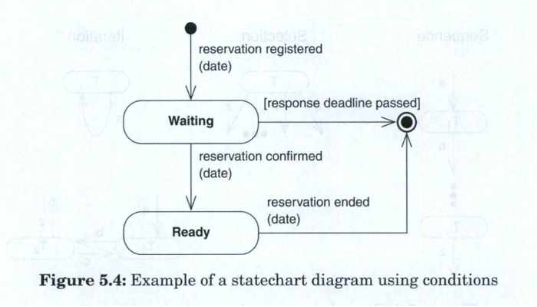
\includegraphics[width=\linewidth]{parts/2_problem_domain_analysis/behavior/figures/condtion_statechart.png}
\end{figure}

\section{Describe Behavioral Patterns \ooad[98]}
In the class activity the connection between classes and events was created in an event table. These unordered events can then be ordered by identifying the first and last events in an objects life.
\begin{itemize}
    \item Which events cause the creation of a problem-domain object? These events are grouped as selections that can cause the birth of an object.
    \item Which events cause the disappearance of a problem-domain object? These events are grouped as selections that can cause the death of an object.
\end{itemize}
An object is birthed when the first event is triggered, and is dead when the last occurs. This does however not mean it ceases to exists, only events cannot occur on it any more.
\\\\
Generally ensure that the problem-domain model includes both structured and unstructured forms of behavioral patterns.

\subsection*{Unstructured}
The unstructured form contains a collection of intermediate events in a combination of selction and iteration. Meaning events can occur an arbitrary amount of times in an arbitrary order.

\subsection*{Structured}
Characterized by an overall sequence, that includes all major events between birth and death. Physical objects and documents are often described this way.
\\\\
When describing behavioral patterns using event traces, ask these questions:
\begin{itemize}
    \item Is the overall form structured or unstructured?
    \item Which events occur together in a sequence?
    \item Are there any alternative events?
    \item Can a given event occur more than once?
\end{itemize}

\subsection*{Sufficient, but Simple \ooad[100]}
Some times conflicting goals:
\begin{itemize}
    \item The behavioral pattern should be sufficiently precise to describe all legal, and thus all illegal, event traces.
    \item The behavioral pattern should provide an overview and thus be as simple as possible.
\end{itemize}
The first goal is to capture all allowable event traces sufficiently, by describing typical behavior.\\
The second goal is to make simple descriptions.
\subsection*{Inheritance of Behavioral Patterns \ooad[102]}
Specialized classes will inherited its super classes behavior, and usually build more sub-patterns on top. Inheritance means it inherites all behavior and their timings.

\section{Explore Patterns \ooad[104]}
Three different models.

\subsection*{The Stepwise Relation Pattern \ooad[104]}
Stepwise relation pattern is used when certain objects are related to the elements of a hierarchy in a stepwise of sequential manner.
\begin{figure}[H]
    \centering
    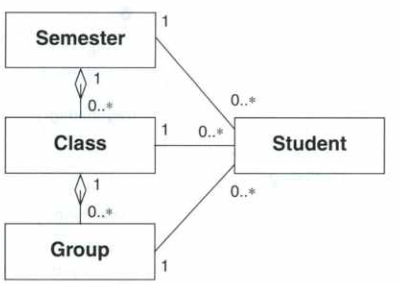
\includegraphics[width=\linewidth/2]{parts/2_problem_domain_analysis/behavior/figures/stepwise_relation.png}
\end{figure}
\subsection*{The Stepwise Role Pattern \ooad[104]} 
\begin{figure}[H]
    \centering
    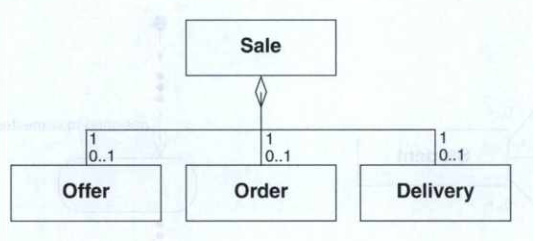
\includegraphics[width=\linewidth/2]{parts/2_problem_domain_analysis/behavior/figures/stepwise_role.png}
\end{figure}

\subsection*{The Composite Pattern \ooad[107]}
The composite pattern offers a way to describe the creation and destruction of a hierarchy using a detailed structure that is unknown at model-development time. 
\begin{figure}[H]
    \centering
    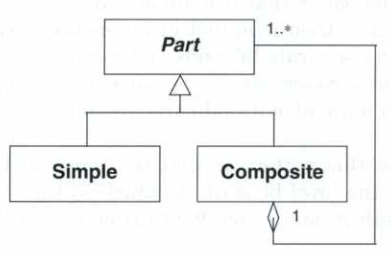
\includegraphics[width=\linewidth/2]{parts/2_problem_domain_analysis/behavior/figures/composite_pattern.png}
\end{figure}

\section{Consider Structure}
\subsection*{Aggregation and Association\ooad[108]}
\begin{itemize}
    \item If two or more objects have common events, consider adding an aggregation or association structure between them.
    \item If two classes are related by an aggregation or association structure, at least one common event should be considered.
\end{itemize}

\subsection*{Generalization \ooad[109]}
\begin{itemize}
    \item If the same event is tied to two classes, consider whether one class is a generalization of the other.
    \item If two classes have many events with the same name, consider whether they are different specializations of a third class.
\end{itemize}